\documentclass{beamer}
\usepackage[utf8]{inputenc}
\usepackage[T1]{fontenc}
\usepackage{lmodern}
\usepackage[english]{babel}
\usepackage{pgf}
\usepackage{units}
\usepackage{lmodern}
\usepackage{color}
\usepackage{listings}
\usepackage{amsmath}
\usepackage[super]{nth}

\newcommand{\notimplies}{%
  \mathrel{{\ooalign{\hidewidth$\not\phantom{=}$\hidewidth\cr$\implies$}}}}

\definecolor{gray}{rgb}{0.5,0.5,0.5}
\definecolor{darkgreen}{rgb}{0.0,0.5,0.0}
\lstset{
  language=C,
  basicstyle=\small\rmfamily,
  numbers=left,
  numberstyle=\tiny\color{gray},
  stepnumber=1,
  numbersep=5pt,
  showspaces=false,
  showstringspaces=false,
  showtabs=false,
  tabsize=8,
  captionpos=b,
  breaklines=true,
  breakautoindent,
  columns=fullflexible,
  morekeywords={inline,bool},
  keywordstyle=\color{blue}\bfseries,
  commentstyle=\color{darkgreen}\itshape,
  stringstyle=\color{magenta}\ttfamily
}
\lstdefinelanguage{diff}{
  morecomment=[f][\color{blue}]{@@},     % group identifier
  morecomment=[f][\color{red}]-,         % deleted lines
  morecomment=[f][\color{darkgreen}]+,   % added lines
  morecomment=[f][\color{magenta}]{---}, % Diff header lines (must appear after +,-)
  morecomment=[f][\color{magenta}]{+++},
}
\def\code{\lstinline[basicstyle=\rmfamily]}

\usetheme{Frankfurt}

% Define the Google colours.
\definecolor{GoogleBlue}{RGB}{0,102,204}
\definecolor{GoogleYellow}{RGB}{255,204,0}
\definecolor{GoogleGreen}{RGB}{0,153,0}
\definecolor{GoogleRed}{RGB}{255,0,0}
\definecolor{GoogleGray}{RGB}{89,89,89}
\newcommand\Google{\href{http://www.google.com/}{%
{\color{GoogleBlue}G}%
{\color{GoogleRed}o}%
{\color{GoogleYellow}o}%
{\color{GoogleBlue}g}%
{\color{GoogleGreen}l}%
{\color{GoogleRed}e}}}

% Use GoogleBlue for all structural text (headers, bullets, etc.)
\setbeamercolor{structure}{fg=GoogleBlue,bg=white}

% Shrink the margins slightly.
\setbeamersize{text margin left=5mm}
\setbeamersize{text margin right=5mm}

% Remove navigation symbols. They are never used anyway.
\setbeamertemplate{navigation symbols}{}

% Make more room on notes pages (when used).
\setbeamertemplate{note page}[plain]
\setbeamerfont{note page}{size=\scriptsize}

% Gray footnotes, no rule.
% FIXME: This is broken. The gray continues onto subsequent slides.
% Note: footnotes are generally a bad idea in presentations.
\setbeamercolor{footnote mark}{fg=GoogleGray}
\renewcommand{\footnoterule}{}

\newcommand\gheaderheight{1mm}
\setbeamertemplate{footline}{%
    \begin{pgfpicture}{0cm}{0cm}{\textwidth}{\gheaderheight}
    \pgfsetcolor{GoogleBlue}
    \pgfrect[fill]{\pgfpoint{0.0\textwidth}{0}}
                  {\pgfpoint{0.25\textwidth}
                  {\gheaderheight}}
    \pgfsetcolor{GoogleRed}
    \pgfrect[fill]{\pgfpoint{0.25\textwidth}{0}}
                  {\pgfpoint{0.25\textwidth}
                  {\gheaderheight}}
    \pgfsetcolor{GoogleYellow}
    \pgfrect[fill]{\pgfpoint{0.50\textwidth}{0}}
                  {\pgfpoint{0.25\textwidth}
                  {\gheaderheight}}
    \pgfsetcolor{GoogleGreen}
    \pgfrect[fill]{\pgfpoint{0.75\textwidth}{0}}
                  {\pgfpoint{0.25\textwidth}
                  {\gheaderheight}}
    \end{pgfpicture}
}


\newcommand\Section[1]{%
\section{#1}%
\begin{frame}%
\frametitle{Outline}
\tableofcontents[currentsection]%,sections=\thesection]%
\end{frame}}


\newcommand\theauthor{Michał Nazarewicz}
\newcommand\theemail{mina86@mina86.com}
\title{Continuous Memory Allocator}
\subtitle{Allocating big chunks of physically contiguous memory}
\author[\theauthor]{%
  \texorpdfstring{\theauthor\vskip 8pt%
    \scriptsize\href{mailto:\theemail}{\theemail}}{%
    \theauthor}}
\institute{\Google}
\date{\today}

\setbeamerfont{institute}{size={\fontsize{10pt}{12pt}}}
\setbeamerfont{date}{size={\fontsize{8pt}{10pt}}}


\begin{document}

\begin{frame}
  \titlepage
\end{frame}

\begin{frame}
  \frametitle{Outline}
  \tableofcontents
\end{frame}

\Section{Introduction}
\subsection{Why physically contiguous memory is needed}

\begin{frame}
  \frametitle{The mighty MMU}

  \begin{itemize}
  \item Modern CPUs have MMU.
    \begin{itemize}
    \item Virtual $\rightarrow$ physical address.
    \end{itemize}
  \item Virtually contiguous $\notimplies$ physically contiguous.
  \item So why bother?
  \end{itemize}
\end{frame}

\begin{frame}
  \frametitle{System devices}

  \begin{itemize}
  \item MMU stands behind CPU.
  \item There are other chips in the system.
  \item Some require large buffers.
    \begin{itemize}
    \item 5-megapixel camera anyone?
    \end{itemize}
  \item On embedded, there's plenty of those.
  \end{itemize}
\end{frame}

\begin{frame}
  \frametitle{The mighty DMA}

  \begin{itemize}
  \item DMA can do vectored I/O.
  \item Gathering buffer from scattered parts.
  \item Contiguous for the device $\notimplies$ physically contiguous.
  \item So why bother?
  \end{itemize}
\end{frame}

\begin{frame}
  \frametitle{The mighty system MMU}

  \begin{itemize}
  \item What about a~system MMU?
    \begin{itemize}
    \item Address coming from the device $\rightarrow$ physical
      address
    \end{itemize}
  \item Same deal as with CPU's MMU.
  \item So why bother?
  \end{itemize}
\end{frame}

\begin{frame}
  \frametitle{Cost, speed \& power}

  \begin{itemize}
  \item Every chip costs.
    \begin{itemize}
    \item Money and power.
    \end{itemize}
  \item More complex chips cost more.
  \item Not all systems have DMA with SG or system MMU.
  \item System MMU takes time.
  \end{itemize}
\end{frame}

% Copyright (c) 2012 by Michał Nazarewicz <mina86@mina86.com>
% Distributed under the terms of the Creative Commons
% Attribution-ShareAlike 3.0 Unported (CC BY-SA 3.0) license.

\subsection{Solutions to the problem}

\begin{frame}
  \frametitle{Lie to the kernel}

  \begin{itemize}
  \item Lie to the kernel about amount of memory.
    \begin{itemize}
    \item Easily done with a~\code{mem} parameter.
    \item Kernel won't touch memory hidden via \code{mem}.
    \end{itemize}
  \item Assign buffers to each device that might need it.
  \item Platform dependent.
  \item Requires fiddling with boot loader.
  \item \ldots
  \end{itemize}
\end{frame}

\begin{frame}
  \frametitle{Reserve and assign at boot time}

  \begin{itemize}
  \item Reserve memory during system boot time.
  \item Assign buffers to each device that might need it.
  \item Less platform dependent.
  \item Boot loader is left alone.
  \item While device is not being used, memory is wasted.
  \end{itemize}
\end{frame}

\begin{frame}
  \frametitle{Reserve but allocate on demand}

  \begin{itemize}
  \item Reserve memory during system boot time.
  \item Provide API for allocating from that reserved pool.
  \item Less memory is reserved.
  \item But it's still wasted.
  \end{itemize}

  \begin{itemize}
  \item bigphysarea
  \item Physical Memory Manager
  \end{itemize}
\end{frame}

\begin{frame}
  \frametitle{Reserve but give back}

  \begin{itemize}
  \item Reserve memory during system boot time.
  \item Give it back
    \begin{itemize}
    \item but set it up so only movable pages can be allocated.
    \end{itemize}
  \item Provide API for allocating from that reserved pool.
  \item Migrate pages on allocation.
  \end{itemize}

  \begin{itemize}
  \item Contiguous Memory Allocator
  \end{itemize}
\end{frame}

\Section{Usage \& Integration}
\subsection{Using CMA from a~device drivers}

\begin{frame}
  \frametitle{Overview}

  \begin{itemize}
  \item CMA is integrated with the DMA API.
  \item If device driver uses the DMA API, nothing needs to be changed.
  \item In fact, device driver should always use the DMA API and never
    call CMA directly.
  \end{itemize}
\end{frame}

\begin{frame}[fragile]
  \frametitle{Allocating memory from device driver}

  \begin{block}{Allocation}
\begin{lstlisting}
void *my_dev_alloc_buffer(
    unsigned long size_in_bytes, dma_addr_t *dma_addrp)
{
    void *virt_addr = dma_alloc_coherent(
        my_dev, size_in_bytes, dma_addrp, GFP_KERNEL);
    if (!virt_addr)
        dev_err(my_dev, "Allocation failed.");
    return virt_addr;
}
\end{lstlisting}
  \end{block}

\end{frame}

\begin{frame}[fragile]
  \frametitle{Releasing memory from device driver}

  \begin{block}{Freeing}
\begin{lstlisting}
void *my_dev_free_buffer(
    unsigned long size, void *virt, dma_addr_t dma)
{
    dma_free_coherent(my_dev, size, virt, dma);
}
\end{lstlisting}
  \end{block}
\end{frame}

\begin{frame}
  \frametitle{Documentation}

  \begin{itemize}
  \item \lstinline|Documentation/DMA-API-HOWTO.txt|
  \item \lstinline|Documentation/DMA-API.txt|
  \item Linux Device Drivers, \nth{3} edition, chapter 15.
    \begin{itemize}
    \item \url{http://lwn.net/Kernel/LDD3/}
    \end{itemize}
  \end{itemize}
\end{frame}

% Copyright (c) 2012 by Michał Nazarewicz <mina86@mina86.com>
% Distributed under the terms of the Creative Commons
% Attribution-ShareAlike 3.0 Unported (CC BY-SA 3.0) license.

\subsection{Integration with the architecture}

\begin{frame}
  \frametitle{Integration with the architecture}

  \begin{itemize}
  \item CMA needs to be integrated with the architecture.
  \item Memory needs to be reserved.
  \item There are early fixups to be done. {\footnotesize Or not.}
  \item The DMA API needs to be made aware of CMA.
  \item And Kconfig needs to be instructed to allow CMA.
  \end{itemize}
\end{frame}

\begin{frame}[fragile]
  \frametitle{Memory reservation}

  \begin{itemize}
  \item \code{memblock} must be ready, page allocator must not.
  \item On ARM, \code{arm_memblock_init()} is a~good place.
  \item All one needs to do, is call
    \code{dma_contiguous_reserve()}.
  \end{itemize}

  \begin{block}{Memory reservation}
\begin{lstlisting}
void __init dma_contiguous_reserve(
    phys_addr_t limit);
\end{lstlisting}
  \end{block}

  \begin{description}[limitAA]
  \item[{\ttfamily limit}] Upper limit of the region (or zero for no
    limit).
  \end{description}

\end{frame}

\begin{frame}[fragile]
  \frametitle{Memory reservation, cont.}

  \begin{block}{Reserving memory on ARM}
\begin{lstlisting}[language=diff]
 if (mdesc->reserve)
     mdesc->reserve();

+/*
+ * reserve memory for DMA contigouos allocations,
+ * must come from DMA area inside low memory
+ */
+dma_contiguous_reserve(min(arm_dma_limit, arm_lowmem_limit));
+
 arm_memblock_steal_permitted = false;
 memblock_allow_resize();
 memblock_dump_all();
\end{lstlisting}
  \end{block}
\end{frame}

\begin{frame}
  \frametitle{Early fixups}

  \begin{itemize}
  \item Kernel linear mapping uses huge pages.
  \item On ARM cache is not coherent.
  \item Having two mappings with different cache-ability gives
    undefined behaviour.
  \item So on ARM an “early fixup” is needed.
    \begin{itemize}
    \item This fixup alters the linear mapping so CMA regions use
      \unit[4]{KiB} pages.
    \end{itemize}
  \item The fixup is defined in
    \code{dma_contiguous_early_fixup()} function
    \begin{itemize}
    \item which architecture needs to provide
    \item with declaration in a~\code{asm/dma-contiguous.h} header file.
    \end{itemize}
  \end{itemize}
\end{frame}

\begin{frame}[fragile]
  \frametitle{Early fixups, cont.}

  \begin{block}{No need for early fixups}
\begin{lstlisting}
#ifndef ASM_DMA_CONTIGUOUS_H
#define ASM_DMA_CONTIGUOUS_H

#ifdef __KERNEL__

#include <linux/types.h>
#include <asm-generic/dma-contiguous.h>

static inline void
dma_contiguous_early_fixup(phys_addr_t base, unsigned long size)
{ /* nop, no need for early fixups */ }

#endif
#endif
\end{lstlisting}
  \end{block}
\end{frame}

\begin{frame}
  \frametitle{Integration with DMA API}

  \begin{itemize}
  \item The DMA API needs to be modified to use CMA.
  \item CMA most likely won't be the only one.
  \end{itemize}
\end{frame}

\begin{frame}[fragile]
  \frametitle{Integration with DMA API}

  \begin{block}{Allocate}
\begin{lstlisting}
struct page *dma_alloc_from_contiguous(
    struct device *dev,
    int count,
    unsigned int align);
\end{lstlisting}
  \end{block}

  \begin{description}[countAA]
  \item[{\ttfamily dev}] Device the allocation is performed on behalf
    of.
  \item[{\ttfamily count}] \emph{Number of pages} to
    allocate. {\footnotesize Not number of bytes nor order.}
  \item[{\ttfamily align}] Order which to align to.  Limited by
    Kconfig option.
  \item Returns page that is the first page of \code{count} allocated
    pages. {\footnotesize It's not a~compound page.}
  \end{description}
\end{frame}

\begin{frame}[fragile]
  \frametitle{Integration with DMA API}

  \begin{block}{Release}
\begin{lstlisting}
bool dma_release_from_contiguous(
    struct device *dev,
    struct page *pages,
    int count);
\end{lstlisting}
  \end{block}

  \begin{description}[countAA]
  \item[{\ttfamily dev}] Device the allocation was performed on behalf
    of.
  \item[{\ttfamily pages}] The first of allocated
    pages. {\footnotesize As returned on allocation.}
  \item[{\ttfamily count}] Number of allocated pages.
  \item Returns \code{true} if memory was freed (ie.\ was managed by
    CMA) or \code{false} otherwise.
  \end{description}
\end{frame}

\begin{frame}
  \frametitle{Let it compile!}

  \begin{itemize}
  \item There's one think that needs to be done in \code{Kconfig}.
  \item Architecture needs to \code{select HAVE_DMA_CONTIGUOUS}.
  \item Without it, CMA won't show up under “Generic Driver Options”.
  \item Architecture may also \code{select CMA} to force CMA in.
  \end{itemize}
\end{frame}

\subsection{Private \& not so private CMA regions}

\begin{frame}
  \frametitle{Default CMA region}

  \begin{itemize}
  \item Memory reserved for CMA is called CMA region or CMA context.
  \item There's one default context devices use.
  \item So why does \code{dma_alloc_from_contiguous()} take
    device as an argument?
  \item There may also be per-device or private contexts.
  \end{itemize}
\end{frame}

\begin{frame}
  \frametitle{What is a~private region for?}

  \begin{itemize}
  \item Separate a~device into its own pool.
    \begin{itemize}
    \item May help with fragmentation.
    \item For instance big vs small allocations.
    \item Several devices may be grouped together.
    \end{itemize}
  \item Use different contexts for different purposes within the same
    device.
    \begin{itemize}
    \item Simulating dual channel memory.
    \item Big and small allocations in the same device.
    \end{itemize}
  \end{itemize}
\end{frame}

\begin{frame}[fragile]
  \frametitle{Declaring private regions}

  \begin{block}{Declaring private regions}
\begin{lstlisting}
int dma_declare_contiguous(
    struct device *dev,
    unsigned long size,
    phys_addr_t base,
    phys_addr_t limit);
\end{lstlisting}
  \end{block}

  \begin{description}[countAA]
  \item[{\ttfamily dev}] Device that will use this region.
  \item[{\ttfamily size}] \emph{Size in bytes} to
    allocate. {\footnotesize Not pagas nor order.}
  \item[{\ttfamily base}] Base address of the region (or zero to use
    anywhere).
  \item[{\ttfamily limit}] Upper limit of the region (or zero for no
    limit).
  \item Returns zero on success, negative error code on failure.
  \end{description}
\end{frame}

\begin{frame}[fragile]
  \frametitle{Region shared by several devices}

  \begin{itemize}
  \item The API allows to assign a~region to a~single device.
  \item What if more than one device is to use the same region.
  \item It can be easily done via “copying” the context pointer.
  \end{itemize}
\end{frame}

\begin{frame}[fragile]
  \frametitle{Region shared by several devices, cont}

  \begin{block}{Copying CMA context pointer between two devices}
\begin{lstlisting}
static int __init foo_set_up_cma_areas(void) {
    struct cma *cma;
    cma = dev_get_cma_area(device1);
    dev_set_cma_area(device2, cma);
    return 0;
}
postcore_initcall(foo_set_up_cma_areas);
\end{lstlisting}
  \end{block}
\end{frame}

\begin{frame}
  \frametitle{Several regions used by the same device}

  \begin{itemize}
  \item CMA uses a~one-to-many mapping from \code{device} structure
    to CMA region.
  \item As such, one device can only use one CMA context\ldots
  \item \ldots unless it uses more than one \code{device}
    structure.
  \item That's exactly what S5PV110's MFC does.
  \end{itemize}
\end{frame}

\Section{Implementation}
\subsection{Page allocator}

\begin{frame}[fragile]
  \frametitle{Pages and page blocks}

  \begin{itemize}
  \item Linux manages memory in units of pages.
    \begin{itemize}
    \item Typically \unit[4]{KiB} in size.
    \end{itemize}
  \item Page can have order ranging from 0 to 10.\footnote{Strictly
    speaking, from zero to one less than \code{MAX_ORDER} which is
    usually 11.}
    \begin{itemize}
    \item $n$-order page consists of $2^n$ \unit[4]{KiB} pages.
    \item 10-order page is called max-order page.
    \end{itemize}
  \item Pages are grouped into page blocks.
  \item Page block consists of 1024 pages, same size as max-order
    page.\footnote{This actually depends, but it's the case for ARM
      and x86.}
  \item {\footnotesize Let's forget about zones or NUMA.}
  \end{itemize}
\end{frame}

\begin{frame}
  \frametitle{Pages and page blocks, cont}
  \begin{center}
  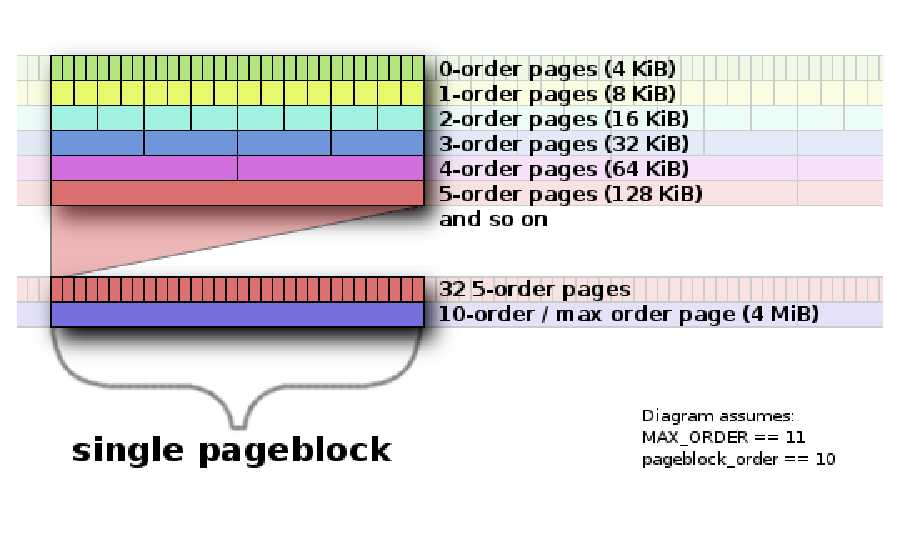
\includegraphics[width=0.9\textwidth]{build/pages.eps}
  \end{center}
\end{frame}

\begin{frame}
  \frametitle{Buddy allocator}
  \begin{columns}[c]

    \column{0.6\textwidth}
    \begin{itemize}
    \item Page allocator uses buddy allocation algorithm.
      \begin{itemize}
      \item Hence different names: buddy system or buddy allocator.
      \end{itemize}
    \item Allocations are done in terms of orders.
    \item User can request order from 0 to 10.
    \item If best matching page is too large, it's recursively split
      in half (into two buddies).
    \item When releasing, page is merged with its buddy (if free).
    \end{itemize}

    \column{0.4\textwidth}
    \begin{center}
    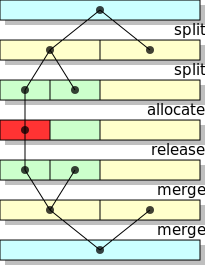
\includegraphics[width=0.9\textwidth]{build/alloc-free-cycle.eps}
    \end{center}
  \end{columns}
\end{frame}

\begin{frame}[fragile]
  \frametitle{Other allocators}

  \begin{itemize}
  \item Page allocator is used for allocations of $2^n$ pages.
  \item For more granular allocations other mechanisms are provided as
    well:
    \begin{itemize}
    \item \code{kmalloc()},
    \item \code{vmalloc()},
    \item Memory pools.
    \end{itemize}
  \item They fall outside of the scope of this presentation.
  \end{itemize}
\end{frame}

\begin{frame}[fragile]
  \frametitle{Migrate types}

  \begin{itemize}
  \item On allocation, user requests an unmovable, a~reclaimable or
    a~movable page.
    \begin{itemize}
    \item For our purposes, we treat reclaimable as unmovable.
    \end{itemize}
  \item To try keep pages of the same type together, each free page
    and each page block has a~migrate type assigned.
    \begin{itemize}
    \item But allocator will use fallback types.
    \item And migrate type of a~free page and page blocks can change.
    \end{itemize}
  \item When released, page takes migrate type of pageblock it belongs
    to.
  \end{itemize}
\end{frame}

\subsection{Page allocator}

\begin{frame}[fragile]
  \frametitle{Pages and page blocks}

  \begin{itemize}
  \item Linux manages memory in units of pages.
    \begin{itemize}
    \item Typically \unit[4]{KiB} in size.
    \end{itemize}
  \item Page can have order ranging from 0 to 10.\footnote{Strictly
    speaking, from zero to one less than \lstinline|MAX_ORDER| which is
    usually 11.}
    \begin{itemize}
    \item $n$-order page consists of $2^n$ \unit[4]{KiB} pages.
    \item 10-order page is called max-order page.
    \end{itemize}
  \item Pages are grouped into page blocks.
  \item Page block consists of 1024 pages, same size as max-order
    page.\footnote{This actually depends, but it's the case for ARM
      and x86.}
  \item {\footnotesize Let's forget about zones or NUMA.}
  \end{itemize}
\end{frame}

\begin{frame}
  \frametitle{Pages and page blocks, cont}
  \begin{center}
  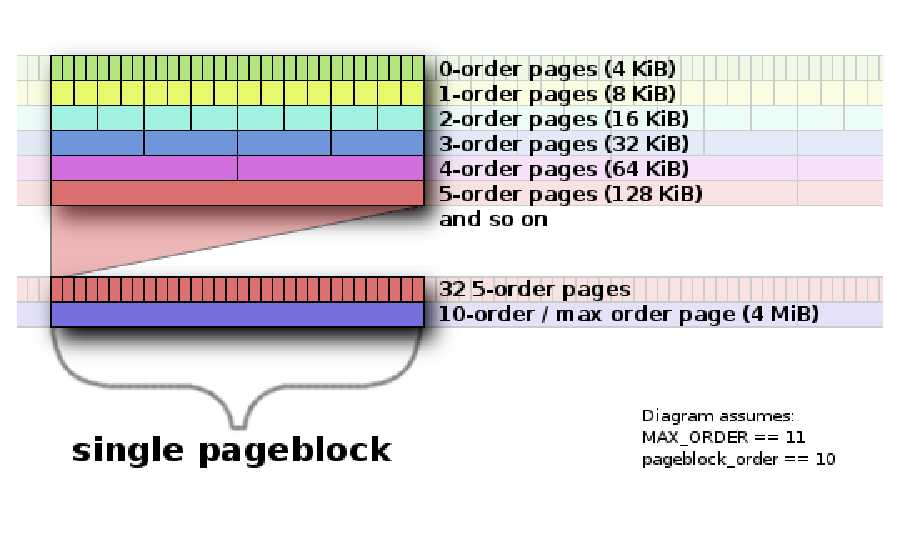
\includegraphics[width=0.9\textwidth]{build/pages.eps}
  \end{center}
\end{frame}

\begin{frame}
  \frametitle{Buddy allocator}
  \begin{columns}[c]

    \column{0.6\textwidth}
    \begin{itemize}
    \item Page allocator uses buddy allocation algorithm.
      \begin{itemize}
      \item Hence different names: buddy system or buddy allocator.
      \end{itemize}
    \item Allocations are done in terms of orders.
    \item User can request order from 0 to 10.
    \item If best matching page is too large, it's recursively split
      in half (into two buddies).
    \item When releasing, page is merged with buddy (if free).
    \end{itemize}

    \column{0.4\textwidth}
    \begin{center}
    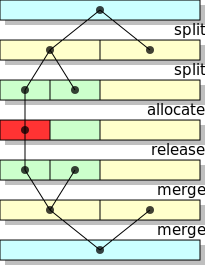
\includegraphics[width=0.9\textwidth]{build/alloc-free-cycle.eps}
    \end{center}
  \end{columns}
\end{frame}

\begin{frame}[fragile]
  \frametitle{Migrate types}

  \begin{itemize}
  \item On allocation, user requests an unmovable, a~reclaimable or
    a~movable page.
    \begin{itemize}
    \item For our purposes, we treat reclaimable as unmovable.
    \end{itemize}
  \item Movable pages will be set up so that they can be migrated.
  \end{itemize}

  \begin{itemize}
  \item To try keep pages of the same type together, each free page
    and each page block has a~migrate type assigned.
  \item But allocator will use fallback types.
  \item And migrate type of a~free page and page blocks can change.
  \end{itemize}
\end{frame}


\appendix

\section*{Q \& A}
\begin{frame}
  \frametitle{Q \& A}

  \begin{center}
  
\includegraphics[width=0.3\textwidth]{build/question.eps}
  \end{center}

  \vskip 2em

  \begin{itemize}
  \item \theauthor
  \item \href{mailto:\theemail}{\theemail}
  \item \url{http://mina86.com/cma/}
  \end{itemize}

  \vskip 2em
  \hfill \includegraphics[height=0.8em,clip=true]{build/cc-by-sa.eps}
\end{frame}

\end{document}
